\begin{frame}{Position Based Separation variables}
	\begin{figure}
		
	% Showing Various Separation
	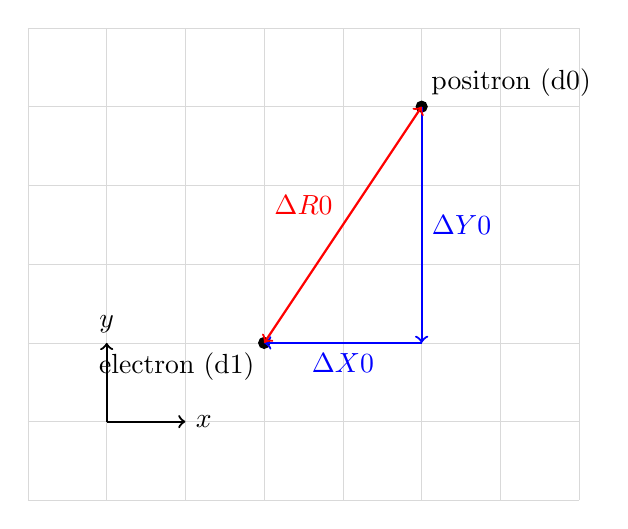
\begin{tikzpicture}[scale=1]
	% Draw grid
	\draw[step=1cm,gray!30,very thin] (-2,-1) grid (5,5);
	
	\coordinate (a) at (1,1);
	\coordinate (b) at (3,4);
	
	% Draw axes
	\draw[->,thick] (-1,0) -- (0,0) node[right] {$x$};
	\draw[->,thick] (-1,0) -- (-1,1) node[above] {$y$};
	% Mark Origin
	% \node[below right] at (0,0) {$(0,0)$};
	
	% Draw and label the points
	\filldraw (a) circle (2pt) node[below left] {electron (d1)};
	\filldraw (b) circle (2pt) node[above right] {positron (d0)};
	
	% Draw delta x, delta y
	\draw[->,thick,blue] (b) -- (a -| b) node[midway,right] {$\Delta Y0$};
	\draw[<-,thick,blue] (a) -- (a -| b) node[midway,below] {$\Delta X0$};
	
	% Draw delta r
	\draw[<->,thick,red] (b) -- (a) node[midway,above left] {$\Delta R0$};
	\end{tikzpicture}
	\caption{Tracking Station 1}
	\end{figure}

	ADD CODE SNIPPET
\end{frame}


\begin{frame}{Track Separation in terms of Momenta [Not Good]}
	\begin{figure}
	\begin{tikzpicture}[scale=1]
		% Define Daughter particles
		\coordinate(d1) at (3, 1);
		\coordinate(d2) at (3, -1);
	
		% Draw grid
		\draw[step=1cm,gray!30,very thin] (1, -3) grid (7, 3);
		\draw[-,thick] (3,-2) -- (3,2) node[pos=0.95, left] {Tracking Station 1};
		\draw[->, thick](3, 0) -- (3.5, 0) node[right] {$z$};
	
		
		% Daughter particles
		\filldraw (d1) circle (2pt) node[below left] {+ve charged (d0)};
		\filldraw (d2) circle (2pt) node[above left] {-ve charged (d1)};
	
		% Make Momentum Vectors
		\draw[->, thick, red]  (d1) -- ($(d1)+(1, 0.5)$) node[right] {$\vec{p_0}$};
		\draw[->, thick, blue] (d2) -- ($(d2)+(1, -0.5)$) node[right] {$\vec{p_1}$};
	
		% Show Translation
		\draw[dashed, red] (d1) -- (4, 0);
		\draw[dashed, red] ($(d1)+(1, 0.5)$) -- ($(4, 0) + (1, 0.5)$);
		\draw[dashed, blue] (d2) -- (4, 0);
		\draw[dashed, blue] ($(d2)+(1, -0.5)$) -- ($(4, 0) + (1,- 0.5)$);
	
		% Show angle between vectors
		\draw[->, thick, red] (4, 0) -- (5, 0.5) node[right] {$\vec{p_1}$};
		\draw[->, thick, blue] (4, 0) -- (5, -0.5) node[right] {$\vec{p_0}$};
		\draw[<->, thick] (4,0) + ({atan(-0.5/1)}:0.6) arc ({atan(-0.5/1)}:{atan(0.5/1)}:0.6) node[midway, right] {$\Phi_p$};
	
	\end{tikzpicture}
	\caption{Angle between Momenta}
	\end{figure}
\end{frame}

\begin{frame}{Track Separation in $\eta$ - $\phi$ Space}
	\begin{figure}
	\begin{tikzpicture}[scale=1]
		% Define Daughter particles
		\coordinate(d1) at (0, 0);
		\coordinate(d2) at (0, 0);
	
		% Draw grid
		\draw[step=1cm,gray!30,very thin] (-1, -2) grid (3, 2);
		\draw[->, thick](-1, -2) -- (2.5, -2) node[right] {$\eta$};
		\draw[->, thick](-1, -2) -- (-1, 2) node[above] {$\phi$};
	
		
		% Daughter particles
		\filldraw (d1) circle (2pt); %node[below left] {+ve charged (d0)};
		\filldraw (d2) circle (2pt); %node[above left] {-ve charged (d1)};
	
		% Make Momentum Vectors
		\draw[->, thick, red]  (d1) -- ($(d1)+(1.5, 1)$) node[right] {$\vec{p_0}$ (d0)};
		\draw[->, thick, blue] (d2) -- ($(d2)+(1.5, -1)$) node[right] {$\vec{p_1}$ (d1)};
		\draw[<->, thick] (0,0) + ({atan(-1/1.5)}:0.6) arc ({atan(-1/1.5)}:{atan(1/1.5)}:0.6) node[midway, right] {$\Delta R_P$};
		
	
	\end{tikzpicture}
	\caption{Angle between Momenta}
	\end{figure}

\end{frame}